\chapter{Review of previous work}

\section{Relevant previous work}
There has been some previous work in the area of automating classification of animal and livestock behaviour using devices attached to animals. Some such relevant work is highlighted in this section. 

Researchers at CSIRO conducted an investigation on the use of Wireless Sensor Networks (WSN) for automated animal monitoring and control \cite{Guo2006}. WSN are made up of sensor nodes that collect sensor data, perform some processing and communicate with other nodes wirelessly. In \cite{Guo2006}, sensor nodes were placed on cattle and data was recorded from accelerometers, magnetometers and GPS. A 10 Hz sampling rate was used to collect data from the accelerometer and magnetometer and this data was then transformed to find such information as heading direction and movement speed. Trends in the data were examined and it was postulated from data analysis that it would be possible to automate the classification of some simple behaviours such as standing and moving for cattle. 

A WSN was also successfully used in a study to classify the behaviour of individual sheep \cite{Nadimi2012}. Sensors were attached to individual sheep and an Artificial Neural Network (ANN), a machine learning technique capable of pattern recognition\footnote{A more detailed introduction to ANNs can be found in section \ref{ANNAppendix}}, was trained with accelerometer data from the sensors that corresponded to behaviour modes of interest. In classifying a range of different modes (grazing, standing etc.), a 76.2\% accuracy was claimed. A higher accuracy was claimed when the classification was simplified to only outputting whether the animal was in an active or inactive state, with a 92.3\% accuracy rate.

When training the ANN it was found that best results (in terms of mean squared error) were achieved using the Nguyen–Widrow and Levenberg–Marquardt back-propagation algorithms. The classification algorithm was not run on the sensors in the WSN but instead sensor values were sent over radio for later classification. This meant that there was considerable power usage; power resources for each node needed to be renovated at the end of each experiment day. During the testing there was a lost packet percentage of 14.8\% overall.

A different machine learning technique, the Support Vector Machine (SVM)\footnote{A more detailed introduction to SVMs can be found in section \ref{SVMAppendix}} was also used to classify the behaviour of free roaming dogs \cite{Gerencser2013}. Videos were used to annotate data recorded from acceleration and gyroscope sensors attached to dogs. The annotated data was then used for training a SVM with good success - a 90\% accuracy was claimed when building a per individual classifier and a 80\% accuracy was claimed when building a generic classifier. 

It was found that the gyroscope data only increased the effectiveness of a recognition system slightly, with the accelerometer data being much more important. To indicate the importance of features for classification, 126 features were extracted from the data and were assigned F-scores. Standard deviation, minimum and maximum were found to be the most relevant feature classes for classification. 

Pattern matching was used in automatically classifying ingestive and ruminative chewing behaviour of cattle using a single axis acceleration sensor \cite{Tani2013}. In this study, sensors were attached in 3 different sites on cattle: the horn, nasal bridge and forehead. However, it was statistically found that the automatic detection rate did not differ significantly between sites. 

The study used stall fed cattle with a claimed accuracy of classification of 90\% but suggested that adapting their method to grazing animals may prove difficult because of the additional animal movement and variety in forage that the animal could eat.

In a paper by Milone et al. Hidden Markov Models (HMMs) were proposed as a method to classify ingestive sounds in sheep \cite{Milone2009}. HMMs are a statistical way of modelling stochastic processes and have previously been used for speech recognition for humans \cite{Milone2009}. In this study, a HMM was defined for each of the events that were to be classified (bite, chew and chew-bite). Gaussian mixture models were used for each state in each HMM to model the spectral features of the audio. Models were created for different heights of pasture, to simulate different grazing conditions so that the complete solution had a HMM for each event and each pasture height. 

An overall performance of 82\% was claimed in the study. It was found that models a with small amount of states worked better than more complicated models. However, modelling states between chewing states proved difficult. Ideally these states would be modelled as silence but background noise causes these states to not be strictly silent. It was postulated that the accuracy would be improved if information about the rate of background noise events could be modelled and included in the classifier. 

Though these machine learning and statistical modelling techniques have proved successful, there has been some research into a time domain approach to quantify the ingestive behaviour of free-grazing cattle \cite{Clapham2011}. Using wide-frequency acoustic microphones that were positioned close to the mouth of cows, signal analysis was performed on the incoming sounds to detect and then measure ingestive events. Recordings were made at 44.1kHz at a 16 bit resolution and then filtered to reduce low frequency noise. 

\begin{figure}[H]
\begin{center}
\leavevmode
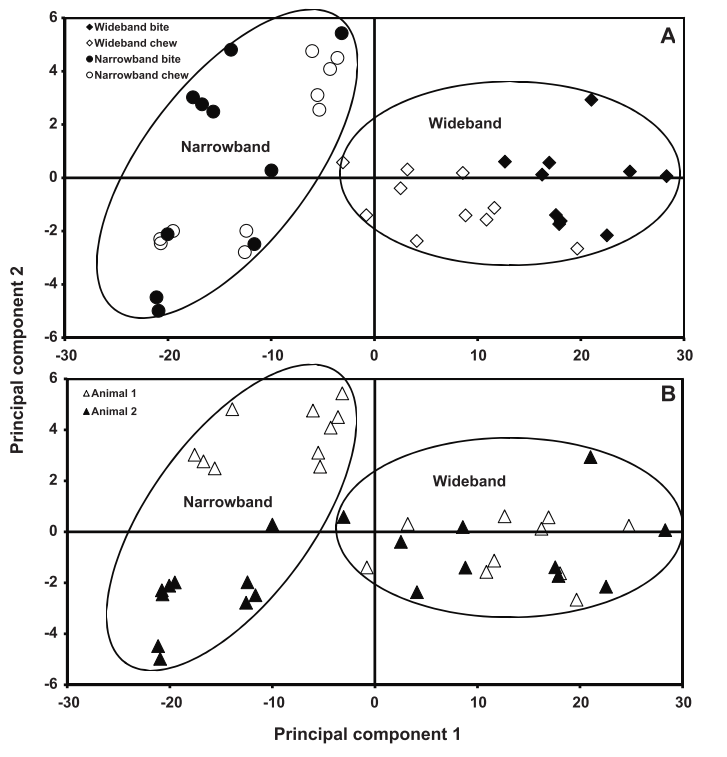
\includegraphics[width=0.6\textwidth]{images/clapham.png}
\end{center}
\caption[PCA of bite/chew frequency spectra]{"Results from principal component analysis of frequency spectra comparing: (a) bites and chews from wideband and narrowband recordings and (b) the same data distinguished according to the two animals used in the analysis" \cite{Clapham2011}. }
\label{clapham}
\end{figure}

The study found that one of the most distinguishing characteristics of a bite was high frequencies from the initial ripping of forage. Energies between 17kHz and 22kHz were considered when looking for bite events and this was shown to be an effective choice as seen in figure \ref{clapham}. The figure shows a principle components analysis comparing a wide-band and narrow-band approach; it can be seen that the wide-band approach would be much better for classifying events as the events cluster more. Thresholding of energy levels in this frequency band of interest was then used to classify bites and distinguish from other spurious events. This achieved a 95 \% claimed accuracy in identifying bites. Additionally it was found that cross-talk from nearby livestock only interfered with classification in a very small amount of cases. 

\section{Impact of previous work}

Machine learning, pattern recognition and thresholding techniques have been used in automating classification of animal behaviour with success as seen in section 2.1; however in these studies the classification was not performed in real time. Having to collect and then later analyse data is cumbersome and does not scale well. It would be more practical to have the classification running independently in real time as the data arrives. Not only does this give up-to-date classification at all times but also assists in the management of livestock as the activity of individual livestock would be observable. 

Because of the free-roaming nature of animals in pasture, the collection of data for classification over a wireless medium is the most practical method. Methods that involve writing information to storage connected to the sensors on the animal exist but are cumbersome as the collection of data cannot be automated. However, sending data at the higher sampling rates needed for classification \cite{Guo2006} \cite{Clapham2011} wirelessly is not feasible. Not only does sending data at these high rates not scale well, as the amount of bandwidth needed increases linearly with the amount of animals being monitored, but this also has negative impacts on the power usage needed \cite{Nadimi2012}. 

Having a classification system that can run continually with very little on-going maintenance needed would be cost effective. Additionally, there is a potential for a non-negligible packet drop-rate when sending data from sensors attached to free-ranging animals over a wireless medium \cite{Nadimi2012}. Therefore, performing classification on the same device that is measuring the signals would be most practical and classification results could be sent rather than the complete sensor data set. This saves power and bandwidth; however add restrictions in computational complexity. The practicality of using a particular classification technique depends on the complexity of the individual technique and whether it is feasible for it to run in real time on a device attached to the animal.

In considering appropriate sensor data to use with such a classification device, both Nadimi et al. and Gerencser et al. recommend against the use of GPS data for a classifier of animal behaviour \cite{Nadimi2012} \cite{Gerencser2013}. GPS has high energy consumption and loss of signal is probable in areas where an animal may be under foliage. Accelerometer and gyroscope signals for classification are stated as being more robust than GPS since the trade off between relative and local data in an accelerometer and gyroscope and absolute and global data in GPS is not worth the added power cost and decrease in reliability \cite{Gerencser2013}.

Additionally, gyroscope information adds little accuracy compared with accelerometer data \cite{Gerencser2013}. For machine learning applications it was found that standard deviation, minimum and maximum values were the most useful \cite{Gerencser2013}. 


\section{Prior work on project}
\label{sec:prior work}
Currently, CSIRO have performed experiments where sensor nodes are deployed on the eartags of cattle. Sensor nodes are capable of collecting sensor data, processing and communicating with other sensor nodes over a network. A collection of sensor nodes communicating wirelessly form a Wireless Sensor Network (WSN). The sensor node eartag platform is based on the 16 bit CC430F5137 microcontroller unit and has a range of sensors including audio, GPS, accelerometer, magnetometer and gyroscope. A photo of the eartag is shown in figure \ref{eartag} and a photo of the eartag attached to a cow is shown in figure \ref{cow}.


\begin{figure}[H]
\centering
\begin{minipage}{.5\textwidth}
  \centering
  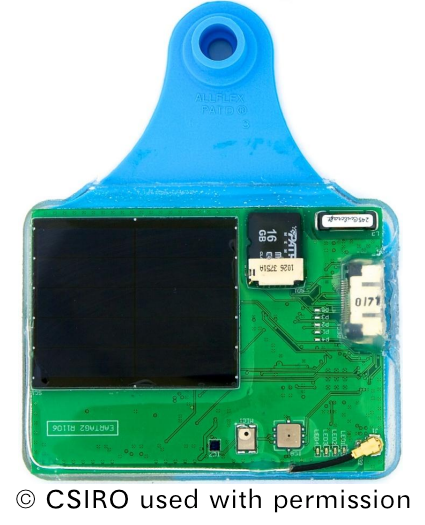
\includegraphics[width=0.4\textwidth]{images/eartag.png}
  \caption{Eartag}
  \label{eartag}
\end{minipage}%
\begin{minipage}{.5\textwidth}
  \centering
  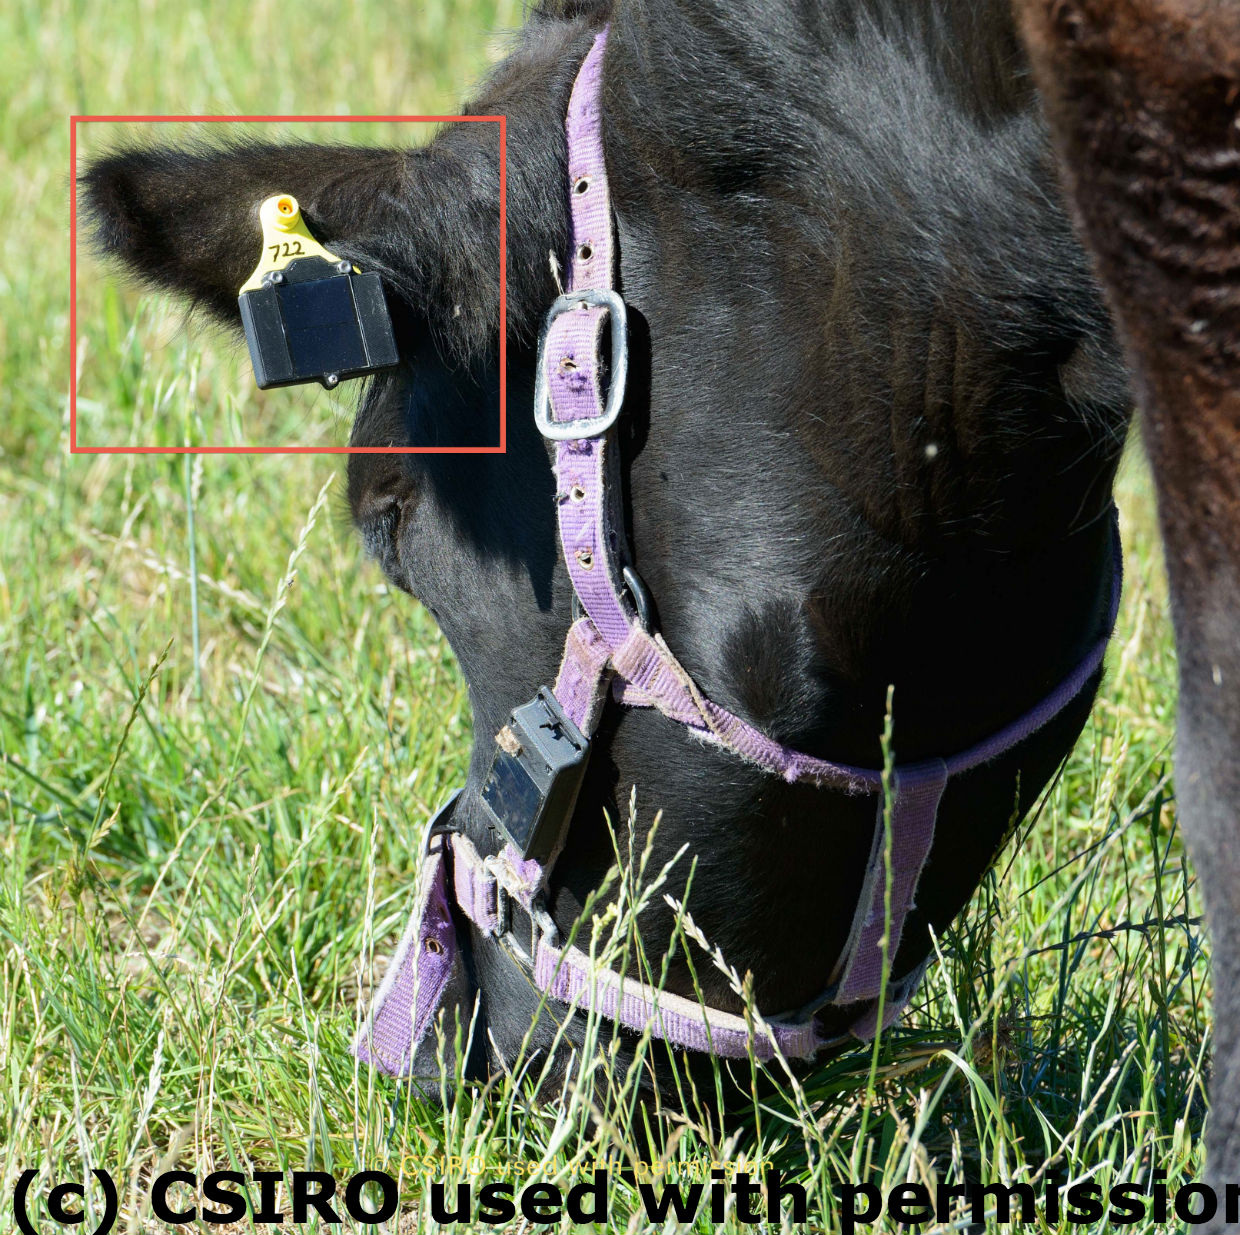
\includegraphics[width=.5\textwidth]{images/cow.jpg}
  \caption{Cow wearing eartag}
  \label{cow}
\end{minipage}
\end{figure}


The WSN platform has been used for animal behaviour classification in the past as seen in section 2.1. It is ideal for the task of real-time classification as sensor nodes are small, low cost, able to communicate wirelessly and run at low power. The eartag platform is powered by a battery and solar panel so that it is possible to run for extended periods. In addition, the sensors nodes are capable of processing so it would be possible to run a classification algorithm on a node. 

CSIRO have performed experiments in a variety of environmental conditions where time-stamped data from sensor nodes attached to cattle is recorded while the cattle behaviour is recorded with video. In this way, data from the eartag can be matched with particular behaviours of the cattle. A classification algorithm can then be designed using this data.